\chapter{Experimental Setup and Results}
This chapter presents the empirical results that validate the decoupled, deep metric learning framework proposed in Chapter 3. Having detailed the systematic methodology, we now turn to the execution and outcomes of the multi-stage evaluation plan. The central objective of this chapter is to systematically assess the performance of each component of the pipeline---from the choice of embedding model and the impact of fine-tuning to the effects of dimensionality reduction and the selection of a downstream classifier---to identify the optimal configuration for both classification accuracy and computational efficiency.

The analysis is structured to first establish the validity of the core feature engineering approach before proceeding through the comparative stages of the evaluation. The chapter begins by detailing the computational environment, datasets, and formal evaluation metrics used throughout the experiments. It then immediately presents a critical ablation study to validate the efficacy of the novel composite distance vector (\(\Delta_c\)), the cornerstone of the feature representation. With the feature vector's design validated, the chapter then follows the primary evaluation sequence: first, establishing a baseline by assessing the performance of various off-the-shelf embedding models and classifiers; second, quantifying the performance gains achieved through fine-tuning; and third, analyzing the trade-offs between accuracy and efficiency introduced by dimensionality reduction. The chapter culminates in a definitive comparative analysis on the held-out test data, synthesizing all prior findings to identify the single best-performing pipeline configuration. We begin by outlining the experimental setup that forms the foundation for all subsequent results.

\section{Experimental Environment \& Datasets}
\subsection{Computational Environment}
The research presented in this thesis was conducted using a hybrid computational environment, leveraging both cloud-based services for initial language model evaluations and a powerful on-premise high-performance computing (HPC) cluster for the primary, computationally intensive experiments. The initial direct classification tasks described in Section 3.1 were performed using Google's Gemini v1.0, a proprietary cloud-based Large Language Model. All subsequent stages of the research, including model fine-tuning, embedding generation, dimensionality reduction, and the comprehensive downstream classifier evaluations, were executed on San Francisco State University's ``POLARIS'' High Performance Compute Cluster.

The POLARIS cluster provided a robust and flexible environment, running on Rocky Linux 8.9 with the Slurm Workload Manager for job scheduling. The GPU-intensive deep learning tasks, particularly the fine-tuning of the embedding models, were performed on the \verb|gpucluster node|. This node is equipped with two AMD EPYC 9334 CPUs (providing 64 cores and 128 threads), 1 TB of RAM, and is accelerated by four NVIDIA A100 GPUs, each with 80 GB of VRAM and supported by CUDA v12.4. The extensive hyperparameter grid searches for the traditional machine learning classifiers were primarily run on the \verb|cpucluster|, which consists of three nodes, each powered by two AMD EPYC 9534 CPUs (128 cores, 256 threads) and containing 576 GB of RAM. The cluster nodes are interconnected with a high-speed InfiniBand 200 Gb/s network, ensuring efficient data transfer during distributed tasks.

The entire experimental pipeline was implemented in Python, with Jupyter Notebooks serving as the primary environment for rapid prototyping, initial data exploration, and results analysis. The core deep learning components were built using PyTorch, with extensive use of the Hugging Face ecosystem, including the \verb|Transformers|, \verb|Sentence-Transformers|, and \verb|Hub| libraries for model access and training. The classical machine learning experiments were conducted using \verb|scikit-learn| and \verb|XGBoost|. Data manipulation and analysis were handled with \verb|numpy| and \verb|pandas|, while \verb|plotly| was used for visualization and \verb|dill| for object serialization.

\subsection{Datasets}
The evolutionary methodology described in Chapter~\ref{ch:3} was developed and validated using two distinct datasets, each serving a critical purpose at different stages of the research. The use of a smaller, initial dataset for prototyping followed by a larger, more comprehensive corpus for final evaluation is a core component of the experimental design. Table~\ref{tbl:datasets} provides a comparative summary of the key characteristics of both datasets used in this research.
\begin{table}[!tb]
    \captionsetup{skip=5pt}
    \centering
    \caption{Summary of Datasets Used in Evaluation}
    \label{tbl:datasets}
    \resizebox{\columnwidth}{!}{
    \begin{tabular}{p{0.2\textwidth} p{0.4\textwidth} p{0.4\textwidth}}
        \toprule
        \textbf{Characteristic} & \textbf{Initial Dataset} & \textbf{PPM Corpus} \\
        \midrule
        \textbf{Source} & Manually curated via ASSIST  & Program Pathways Mapper (PPM)  \\
        \addlinespace
        \textbf{Purpose} & Preliminary screening, prototyping, and initial classifier evaluation  & Definitive fine-tuning and final pipeline evaluation  \\
        \addlinespace
        \textbf{Ground Truth} & Established articulation agreements  & Course Identification Number (C-ID)  \\
        \addlinespace
        \textbf{Final Size} & 400 course pairs (for evaluation set)  & 2,157 courses (across 157 classes)  \\
        \addlinespace
        \textbf{Partitioning} & Stratified random sample  & Stratified 50/50 train/test split  \\
        \bottomrule
    \end{tabular}
    }
\end{table}
\subsubsection{Initial Dataset}
The first dataset, hereafter referred to as the Initial Dataset, was a manually curated corpus used for the preliminary investigations in Stages 1 and 2 of the evaluation framework. This dataset was constructed from five lower-division courses at San Francisco State University and their established articulation agreements from 63 other California public colleges, sourced via the ASSIST repository. It was used to establish the initial performance baseline with the direct LLM classification approach and to prototype the decoupled pipeline. The final evaluation set for these preliminary stages consisted of a balanced, stratified random sample of 400 course pairs drawn from a larger set of over 11,000 generated pairs.

\subsubsection{PPM Corpus}
The primary and definitive experiments for this thesis were conducted on the PPM Corpus, a larger and more robust dataset provided by the Program Pathways Mapper (PPM). This corpus served as the foundation for the full-scale implementation, fine-tuning, and final validation of the decoupled pipeline (Stages 3 and 4). After a filtering process detailed in Section~\ref{ch:3.2.1}, the final corpus consists of 2,157 courses, each labeled with a Course Identification Number (C-ID) that serves as the ground truth for equivalency. This corpus was partitioned via a stratified 50/50 split into a training set of 1,078 courses and a held-out test set of 1,079 courses. This held-out test set is crucial for methodological rigor and was used only once for the final, conclusive evaluation of the optimized pipelines to provide an honest and unbiased estimate of their generalization performance.

\subsection{Evaluation Metrics}
To facilitate a comprehensive and multi-faceted analysis, a suite of standard evaluation metrics was used to assess the various pipeline configurations. These metrics were chosen to measure performance across two critical dimensions: classification efficacy and computational efficiency, ensuring that the final recommended pipeline is not only accurate but also practical for real-world deployment.

\subsubsection{Classification Efficacy}
The core assessment of classification performance is based on a standard suite of metrics derived from the confusion matrix, which tabulates the counts of True Positives (\(TP\)), True Negatives (\(TN\)), False Positives (\(FP\)), and False Negatives (\(FN\)). While Accuracy, defined as \(\frac{TP + TN}{TP + TN + FP + FN}\), provides a general overview of correctness, it can be insufficient for capturing the nuances of a classifier's behavior. Therefore, this research also evaluates:
\begin{itemize}
    \item \textbf{Precision}: Calculated as \(\frac{TP}{TP + FP}\), this metric measures a model's exactness. High precision indicates that when the model predicts an equivalency, it is likely to be correct.
    \item \textbf{Recall}: Calculated as \(\frac{TP}{TP + FN}\), this metric measures a model's completeness. High recall indicates that the model is effective at identifying the full set of all true equivalencies.
\end{itemize}
The \(F_1\)-Score, the harmonic mean of Precision and Recall (\(2\cdot\frac{Precision\cdot Recall}{Precision + Recall}\)), is used as the primary metric for reporting and comparing the final classification performance. The \(F_1\)-Score provides a single, robust value that balances the trade-off between precision and recall, making it an ideal metric for this task where both avoiding false equivalencies and identifying all true ones are important.

\subsubsection{Efficiency Metric}
Beyond classification efficacy, the practical viability of each pipeline was assessed by measuring its computational efficiency. Both Training Time and Inference Time were systematically captured during the hyperparameter tuning process using the detailed statistics provided by \verb|scikit-learn| \!\!'s \verb|GridSearchCV| utility. Training time reflects the resources required to fit a model configuration, offering insight into the cost of experimentation. Inference time, reported by \verb|GridSearchCV| as \verb|score_time|, measures the time required for a trained model to make predictions on new data. For the use case of this research, inference time is considered the more critical efficiency metric, as it directly impacts the system's real-world responsiveness and scalability in a production environment. Finally, for the specific task of monitoring model improvement during the fine-tuning process (Stage 3), a specialized metric, Average Precision based on cosine similarity, was employed by the \verb|BinaryClassificationEvaluator| to select the best-performing model checkpoint.

\section{Direct LLM Classification}
The initial phase of this research sought to establish a performance baseline by evaluating the feasibility of using a Large Language Model for end-to-end course equivalency classification. The experiments were conducted using the Initial Dataset, a balanced 400-pair sample, and leveraged Google's Gemini Pro v1.0 as the reasoning engine. The evaluation was designed to test two key conditions: the impact of input data type (full raw text vs.\ extracted topics) and the effect of different classification schemes (binary, 3-way, and 4-way) on the model's performance and behavior.

The classification results were encouraging, with the model achieving a peak accuracy of 90.5\% in the binary task using raw text. A primary finding from this phase was that using the full, unprocessed raw text consistently yielded superior results compared to using only the extracted structured topics. This performance gap is likely attributable to the challenges inherent in the data extraction step itself. The process of deducing structured topics from unstructured text proved to be the most time-consuming and difficult aspect of this initial approach, requiring two to four times more time than the classification task and exhibiting a high sensitivity to prompt wording—a finding that aligns with previous studies on prompt engineering by Sclar et al., Errica et al., Chen et al., Cheung, and Gerych et al.~\cite{Sclar2023QuantifyingLM,Errica2024WhatDI,Chen2024LLMAA,Cheung2024ARC,Gerych2024WhoKT}. Although Gemini demonstrated a general capability to understand the context of the course descriptions, its limitations in flawlessly deducing course topics appear to have introduced enough noise to degrade the performance of the topics-based classification.

An analysis of the confusion matrices, presented in Figure~\ref{fig:cm} reveals a consistent and telling behavioral pattern: the model exhibits a strong conservative bias. Across all scenarios, the ``not equivalent'' class showed higher recall than precision, while the ``equivalent'' class showed higher precision than recall. For example, in the binary raw text evaluation, the model produced 34 false negatives but only 4 false positives. This indicates that the model is far more likely to misclassify a truly equivalent course as ``not equivalent'' than it is to incorrectly approve a non-equivalent pair. This conservative tendency suggests the LLM operates with a high internal threshold for declaring equivalency, preferring to err on the side of caution.
\begin{figure}[tb]
    \captionsetup{skip=5pt}
    \centering
    \begin{subfigure}[b]{0.45\textwidth}
        \centering
        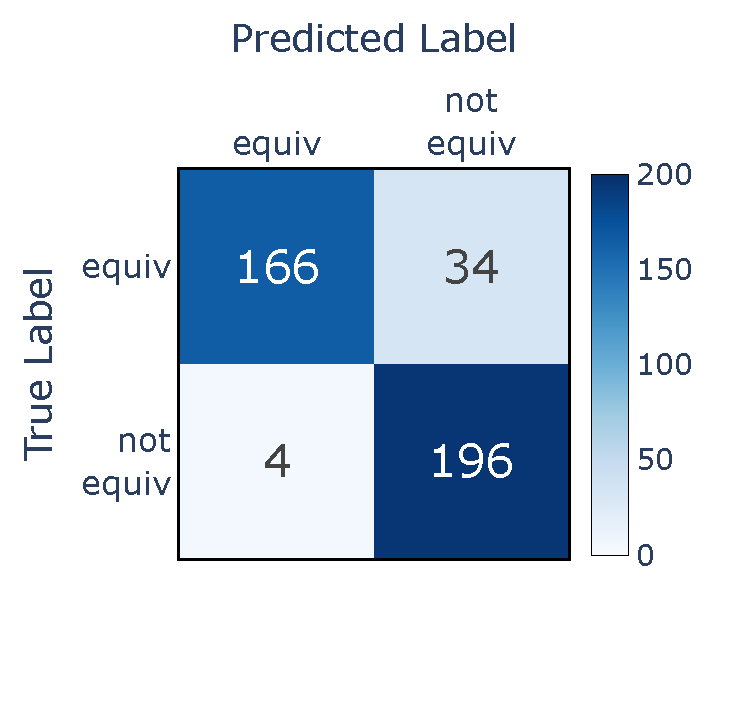
\includegraphics[scale=0.41,trim={3mm 20mm 7mm 0},clip]{LLMeval_binary_raw_text_cm.pdf}
        \caption{Binary Raw Text}
        \label{fig:sub_brt}
    \end{subfigure}
    \hfill
    \begin{subfigure}[b]{0.45\textwidth}
        \centering
        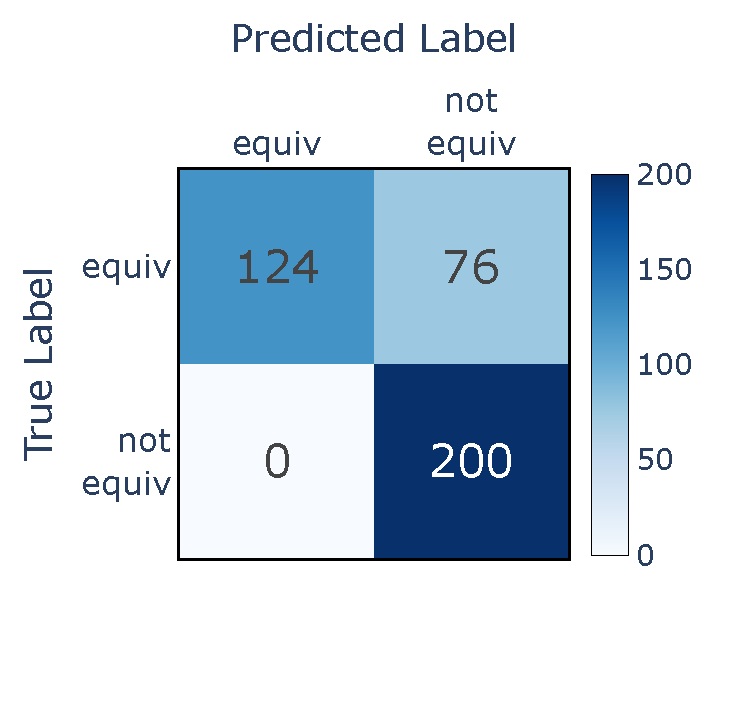
\includegraphics[scale=0.41,trim={3mm 20mm 7mm 0},clip]{LLMeval_binary_topics_cm.pdf}
        \caption{Binary Topics}
        \label{fig:sub_brt}
    \end{subfigure}

    \vspace{2mm}

    \begin{subfigure}[b]{0.45\textwidth}
        \centering
        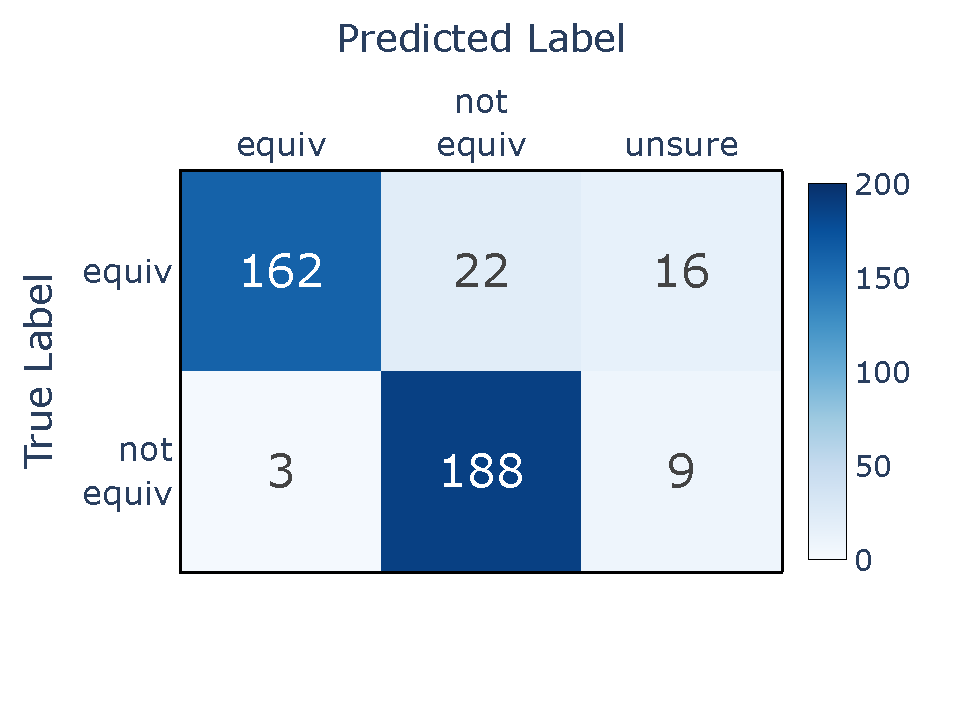
\includegraphics[scale=0.41,trim={3mm 20mm 7mm 0},clip]{LLMeval_3way_raw_text_cm.pdf}
        \caption{3-way Raw Text}
        \label{fig:sub_brt}
    \end{subfigure}
    \hfill
    \begin{subfigure}[b]{0.45\textwidth}
        \centering
        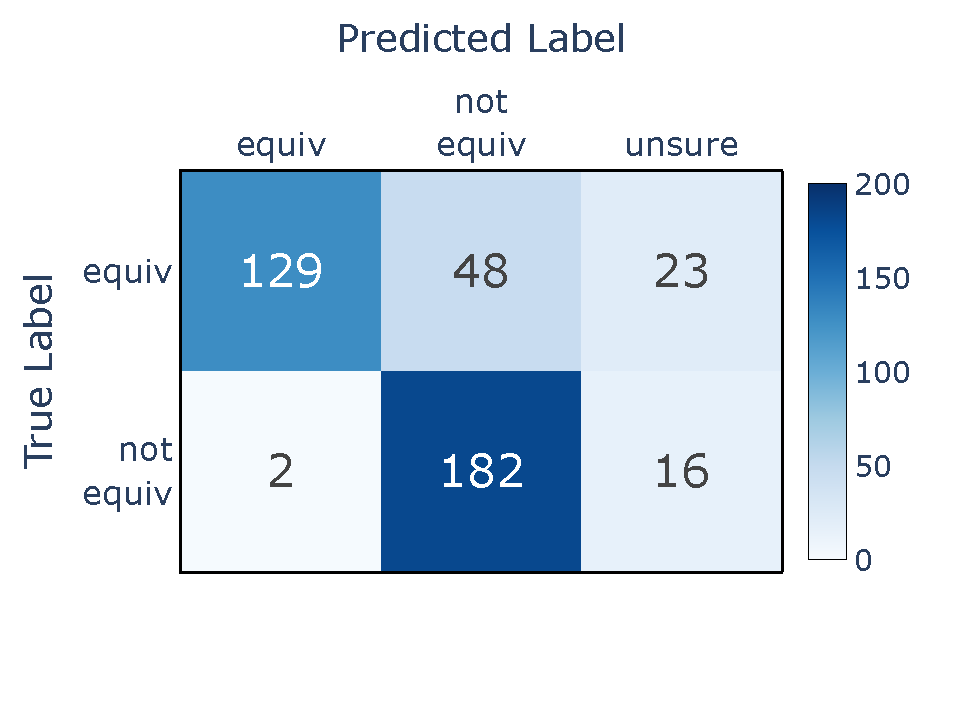
\includegraphics[scale=0.41,trim={3mm 20mm 7mm 0},clip]{LLMeval_3way_topics_cm.pdf}
        \caption{3-way Topics}
        \label{fig:sub_brt}
    \end{subfigure}

    \vspace{2mm}

    \begin{subfigure}[b]{0.45\textwidth}
        \centering
        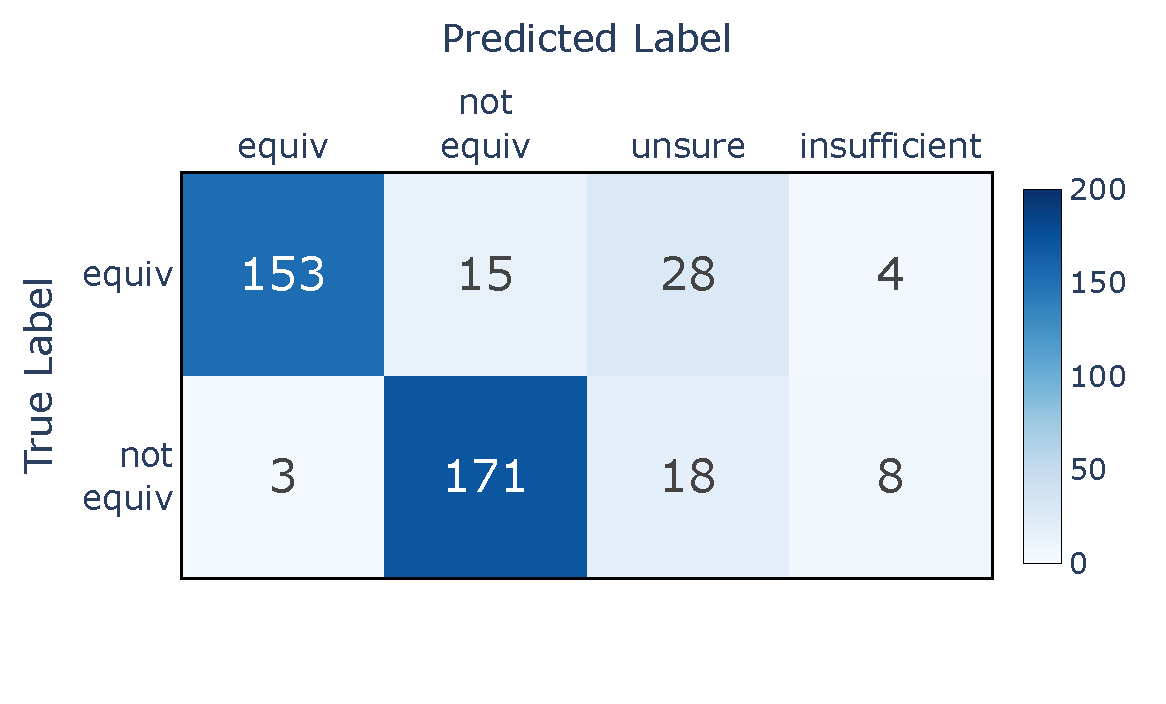
\includegraphics[scale=0.41,trim={3mm 20mm 7mm 0},clip]{LLMeval_4way_raw_text_cm.pdf}
        \caption{4-way Raw Text}
        \label{fig:sub_brt}
    \end{subfigure}
    \hfill
    \begin{subfigure}[b]{0.45\textwidth}
        \centering
        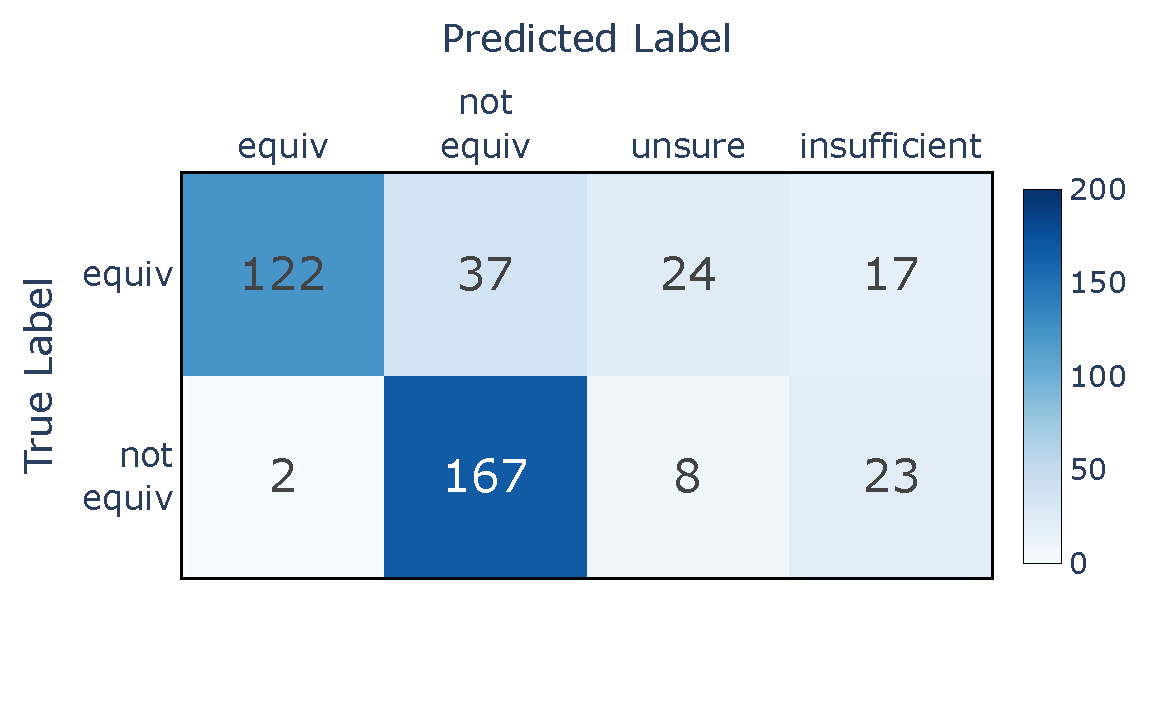
\includegraphics[scale=0.41,trim={3mm 20mm 7mm 0},clip]{LLMeval_4way_topics_cm.pdf}
        \caption{4-way Topics}
        \label{fig:sub_brt}
    \end{subfigure}
    \caption{LLM Classification Confusion Matrices}
    % {\footnotesize Clockwise from bottom left: 4-class raw text, 3-class raw text, binary raw text, binary
    %     structured topics, 3-class structured topics, and 4-class structured topics.\\\footnotemark[1]ins: insufficient description}
    \label{fig:cm}
\end{figure}

The introduction of the ``unsure'' and ``insufficient data'' categories was designed to simulate how a human advisor might handle ambiguity. While there is no ground truth for these labels, their value lies in the model's ability to isolate cases that require further manual review. This is particularly relevant for courses that may have significant topical overlap but different learning outcomes, or for descriptions that are too sparse to allow for a definitive decision. For instance, in the 4-way raw text evaluation, the model flagged 46 pairs as ``unsure'' and 12 as having ``insufficient'' information, effectively separating these ambiguous cases from the main classification flow.  Table~\ref{tbl:llm_results_summary} provides a comprehensive summary of the performance metrics for all six experimental conditions.
\begin{table}[!tb]
    \captionsetup{skip=5pt}
    \centering
    \caption{Performance Summary of Direct LLM Classification}
    \label{tbl:llm_results_summary}
    \begin{tabular}{lccccc}
        \toprule
        & \textbf{Classification} & & & & \\
        \textbf{Input Data} & \textbf{Task} & \textbf{Accuracy} & \textbf{F1-Score*} & \textbf{Precision*} & \textbf{Recall*} \\
        \midrule
        \multirow{3}{*}{Raw Text} & Binary & 0.9050 & 0.8973 & 0.9765 & 0.8300 \\
        & 3-way & 0.8750 & 0.8877 & 0.9818 & 0.8100 \\
        & 4-way & 0.8100 & 0.8596 & 0.9808 & 0.7650 \\
        \midrule
        \multirow{3}{*}{Topics} & Binary & 0.8100 & 0.7654 & 1.0000 & 0.6200 \\
        & 3-way & 0.7775 & 0.7795 & 0.9847 & 0.6450 \\
        & 4-way & 0.7225 & 0.7531 & 0.9839 & 0.6100 \\
        \bottomrule
        \multicolumn{6}{p{0.9\textwidth}}{\scriptsize * F1-Score, Precision, and Recall are reported for the positive class (``Equivalent'').} \\
    \end{tabular}
\end{table}

To contextualize the performance of Gemini Pro, a comparative analysis was conducted against a suite of other prominent open-source LLMs (see Table~\ref{tbl:cls} for a summary of their specifications and performance). The results of this benchmark revealed that Gemini Pro v1.0 outperformed all other models tested. While most models were able to complete the task, their performance varied significantly. The strongest competitor was Anthracite Magnum v1 72B, which achieved a respectable accuracy of 85.25\%, but still falling short of Gemini's 90.5\%.
\begin{table*}[tb]
    \captionsetup{skip=5pt}
    \caption{Model Specifications and Performance}
    \label{tbl:cls}
    \centering
    \resizebox{\columnwidth}{!}{
    \begin{tabular}{lccccccc}
        \toprule
        &  & \textbf{Context} &  &  &
                     &      &      \\
        \textbf{Model Name}             & \textbf{Parameters*} & \textbf{Length} & \textbf{Support} & \textbf{Accuracy} &
        \textbf{Precision}              & \textbf{Recall}      & \(\mathbf{F_1}\)\textbf{-score}                                                                                                \\
        \midrule
        Google Gemini Pro 1.0           & Unknown              & 32,768                  & 400              & \textbf{0.9050}   & 0.9765 & \textbf{0.8300} & \textbf{0.8973} \\
        Meta Llama 3.1 8B Instruct      & 8                    & 128,000                 & 208 (52\%)       & 0.6250            & 1.0000 & 0.3500          & 0.5185          \\
        Microsoft Phi 3 Medium Instruct & 14                   & 128,000                 & 400              & 0.7100            & 1.0000 & 0.4200          & 0.5915          \\
        Google Gemma 2 27b              & 27.2                 & 8,000                   & N/A              & N/A               & N/A    & N/A             & N/A             \\
        Meta Llama 3.1 70B Instruct     & 70                   & 128,000                 & 400              & 0.7350            & 1.0000 & 0.4700          & 0.6395          \\
        Qwen 2 72B Instruct             & 72.7                 & 131,072                 & 400              & 0.7650            & 1.0000 & 0.5300          & 0.6928          \\
        Anthracite Magnum v1 72B        & 72.7                 & 32,768                  & 400              & 0.8525            & 1.0000 & 0.7050          & 0.8270          \\
        CalmeRys 78B Orpo v0.1          & 78                   & 32,768                  & 400              & 0.7175            & 1.0000 & 0.4350          & 0.6063          \\
        Mixtral 8x22B Instruct v0.1     & 141                  & 65,536                  & 400              & 0.6450            & 1.0000 & 0.2900          & 0.4496          \\
        Meta Llama 3.1 405B Instruct**  & 405                  & 128,000                 & 400              & 0.7775            & 1.0000 & 0.5550          & 0.7138          \\
        \bottomrule
        \multicolumn{8}{l}{\footnotesize *in Billions}                                                                                                                       \\
        \multicolumn{8}{l}{\footnotesize **INT4 Quantized Model}
    \end{tabular}
    }
\end{table*}

This benchmark also highlighted significant operational challenges. Several models struggled to reliably produce valid output. For example, Google's Gemma 2 27B consistently generated unintelligible or irrelevant responses, preventing the collection of any meaningful performance data. Similarly, Meta's Llama 3.1 8B Instruct model was only able to respond correctly to approximately 52\% of the prompts, making it too unreliable for practical use. A surprising insight from this analysis was the lack of a strong correlation between model size and performance on this task. It is important to note, however, that the prompts used in this evaluation were originally designed and optimized for Gemini. This lack of prompt specificity for the other models may have contributed to their lower accuracy and, in some cases, their inability to respond appropriately.

This initial study confirmed that direct LLM classification can achieve high accuracy but is sensitive to input quality and exhibits a conservative bias. More importantly, it validated the fundamental limitations of the approach, its computational cost, lack of a quantifiable similarity score, and ``black box'' nature, that motivated the development of the decoupled pipeline. The following sections will now present the results of this more advanced framework, beginning with a critical validation of its most novel component: the composite distance vector.

\section{Composite Distance Vector Validation}
A foundational contribution of this research is the design of the composite distance vector, \(\Delta_c\), which serves as the input for all downstream classifiers. As detailed in the methodology, this vector was designed to provide a richer feature set than a single similarity score alone by combining granular, dimension-specific (local) information with a holistic, global similarity metric . This section presents the results of a critical ablation study designed to validate this hypothesis and quantify the impact of the global cosine similarity term on classifier performance.

The experimental setup for this validation involved training the full suite of classifiers on two different versions of the feature set. The first used the complete composite distance vector (\(\Delta_c\)), which includes both the element-wise differences and the cosine similarity score. The second used an ablated vector (\(\Delta_l\)) containing only the element-wise differences. By comparing the performance across these two conditions, it is possible to isolate and measure the contribution of the global similarity feature.

The results of this ablation study revealed a stark and significant dichotomy between the behavior of linear and non-linear models. For all linear models evaluated—Logistic Regression, Ridge Regression, Lasso, and Linear Discriminant Analysis (LDA), the inclusion of the cosine similarity term resulted in a dramatic and statistically significant improvement in classification performance. For example, using the off-the-shelf BGE embeddings with no dimensionality reduction, the F1-score for the Logistic Regression classifier surged from 0.686 to 0.901 with the addition of the single cosine similarity feature. This massive performance lift demonstrates that for these simpler models, which are constrained to learning linear decision boundaries, the explicit global similarity feature provides critical information that they are unable to derive from the local element-wise differences alone.

In stark contrast, the more complex non-linear models, \(k\)-Nearest Neighbors (KNN), Support Vector Machine (SVM), and Random Forest (RF), were not significantly influenced by the inclusion or omission of the cosine similarity term. Their performance remained exceptionally high in both conditions. For instance, the \(F_1\)-score for the SVM classifier was virtually unchanged, registering 0.9988 without the term and 0.9983 with it. This suggests that these more powerful models, which can learn complex, non-linear interactions between features, are capable of effectively reconstructing the global similarity information directly from the high-dimensional local difference vector.

The conclusion from this ablation study is clear and decisive. The composite distance vector, \(\Delta_c\), is demonstrably the superior feature representation. It provides a critical performance boost to simpler, baseline models while causing no harm to the performance of more sophisticated, non-linear models. Therefore, based on this empirical validation, the full composite distance vector was adopted as the standard feature set for all subsequent experiments presented in this thesis.

\section{Fine-Tuning a Model}
This section details the empirical investigation into enhancing the performance of pre-trained embedding models by fine-tuning them on the domain-specific PPM Corpus. The central hypothesis, as stated in Section~\ref{ch:3.3}, is that adapting a general-purpose model to the specific linguistic nuances of course catalog text will yield a more discriminative feature representation for the downstream course equivalency task. This process, a form of deep metric learning, aims to restructure the embedding space such that the geometric distance between vectors directly corresponds to semantic similarity. Such an approach is particularly relevant for scenarios with high intra-class variance and low inter-class variance, a common characteristic of specialized domains where fine distinctions are paramount. This section outlines the rigorous experimental design, presents the empirical results, and provides a detailed analysis that culminates in the selection of a single, optimized model for subsequent evaluation.

\subsection{Evaluation Framework}
To identify the optimal fine-tuning configuration, a systematic evaluation was designed and executed, exploring a matrix of key hyperparameters. The experimental runs were orchestrated via a series of shell scripts that automated the submission of training jobs with different configurations. This framework was designed to methodically test the impact of different loss functions and learning rate schedules on model performance.  
\begin{itemize}
    \item \textbf{Base Models}: The experiments focused on fine-tuning the most promising small model identified in the initial screening (Section~\ref{ch:3.3}): \verb|BAAI/bge-small-en-v1.5| (BGE). This model was selected to represent high-performing small architecture.
    \item \textbf{Loss Functions}: A critical component of metric learning is the choice of the loss function, which defines the optimization objective. This study evaluated four distinct online triplet mining strategies, each implemented as a loss function within the sentence-transformers library. The selection of a loss function directly influences which training examples are considered most informative, impacting both convergence speed and final model performance. The evaluated functions were:  
    \begin{itemize}
        \item \textbf{BatchAllTripletLoss (atl)}: Computes the loss over all valid triplets within a mini-batch, offering a comprehensive but potentially diluted learning signal.
        \item \textbf{BatchSemiHardTripletLoss (shtl)}: Considers only semi-hard triplets, where the negative sample is more distant than the positive but still violates the margin. This is a common strategy that balances stability and learning effectiveness.
        \item \textbf{BatchHardTripletLoss (htl)}: Focuses on the hardest triplets in each batch, providing a strong but potentially unstable learning signal by using the most challenging examples.  
        \item \textbf{BatchHardSoftMarginTripletLoss (hsmtl)}: A variation of \verb|BatchHardTripletLoss| that does not require a fixed margin parameter, simplifying hyperparameter tuning.
    \end{itemize}
    \item \textbf{Learning Rate Schedulers}: The learning rate schedule governs how the learning rate is adjusted during training, a critical factor for navigating complex loss landscapes and avoiding premature convergence. Three distinct schedules, with parameters defined in the training script, were evaluated.
    \begin{itemize}
        \item \textbf{linear (lr\_linear)}: A standard linear decay of the learning rate from its initial value to zero over the course of training.
        \item \textbf{cosine\_with\_restarts (cr\_v1)}: A cosine annealing schedule with 6 restart cycles and an early stopping patience of 21 epochs.
        \item \textbf{cosine\_with\_restarts (cr\_v2)}: A more aggressive cosine annealing schedule with 10 restart cycles and a reduced early stopping patience of 15 epochs.
    \end{itemize}
\end{itemize}
The dynamic behavior of these schedulers, particularly the periodic resets of the cosine annealing schedules, is visualized in the training logs, confirming their implementation as designed (Image 1).

\subsection{Implementation Details}
The fine-tuning experiments were conducted with a high degree of methodological rigor, leveraging a sophisticated distributed training environment and custom tools to ensure robustness and reproducibility. The computationally intensive nature of fine-tuning transformer models necessitated the use of a high-performance computing (HPC) environment. All experiments were executed on the POLARIS HPC cluster at San Francisco State University. The SLURM submission script specifies a distributed data-parallel (DDP) strategy using \verb|torchrun| with a configuration of \verb|nproc_per_node=4|, distributing the workload across four NVIDIA A100 GPUs on a single node. This setup significantly accelerated the training process, making the comprehensive grid search feasible.

The choice of a data batching strategy is intrinsically linked to the mechanics of the loss function. The batch-based triplet loss functions perform ``online'' mining, meaning they construct informative (anchor, positive, negative) triplets on-the-fly from the samples present within each training mini-batch. For a valid triplet to be formed, the batch must contain at least two examples from the same class, enabling the selection of a distinct anchor and positive sample. Standard random sampling does not guarantee this condition, which can lead to inefficient training where many anchors in a batch cannot form valid triplets. To address this, the \verb|GroupByLabelBatchSampler| class was employed, as specified in the training script. This sampler, a feature of the \verb|sentence-transformers| library, ensures that each mini-batch is constructed by grouping multiple samples with the same label. This guarantees that every batch contains the necessary class diversity to form valid and informative triplets for all anchors, maximizing the utility of each training step.  

To manage the long-running, distributed training jobs, a set of custom \verb|TrainerCallback| classes were implemented. The \verb|DistributedStoppingCallback| is particularly significant as it demonstrates a sophisticated approach to process control in a distributed setting. This callback integrates two crucial features: early stopping based on a patience parameter (i.e., halting training if the validation metric does not improve for a set number of evaluations) and a hard time limit (\verb|max_duration|) to ensure jobs do not exceed their allocated time on the HPC cluster. The callback is designed to perform these checks on the main process (rank 0) during the evaluation phase and then broadcast a stop signal to all other worker processes. This architecture prevents the common issue of hanging processes in distributed training and ensures a graceful, synchronized termination of the job, underscoring the methodological robustness of the experimental setup.

The performance of the model during the fine-tuning process was monitored at the end of each epoch using the \verb|BinaryClassificationEvaluator| from the \verb|sentence-transformers| library. The metric used to identify and save the best-performing model checkpoint was the \(F_1\)-score on a binary classification task, specifically \verb|eval_binary classification evaluator_cosine_f1|. This represents a deliberate and important design choice. By training the model to optimize a triplet loss objective while evaluating its performance on a binary pair classification task, the framework directly measures the model's aptitude for the ultimate downstream task. This prevents overfitting to the specific mechanics of the triplet loss and provides a more honest assessment of the model's ability to generalize.

\subsection{Empirical Results of Fine-Tuning Configurations}
The systematic evaluation of the twelve fine-tuning configurations (four loss functions crossed with three learning rate schedules) on the BGE base model produced a rich set of performance data. The training progress was logged and visualized, allowing for both qualitative and quantitative analysis of the different strategies.

\subsubsection{Visualization of Training Dynamics}
Figure~\ref{fig:binaryf1} presents the validation \(F_1\)-score, calculated on the binary classification evaluation task, as a function of the global training step for each of the twelve experimental runs. This visualization provides a clear, qualitative comparison of the learning dynamics associated with each configuration.
\begin{figure}[tb]
    \captionsetup{skip=5pt}
    \centering
    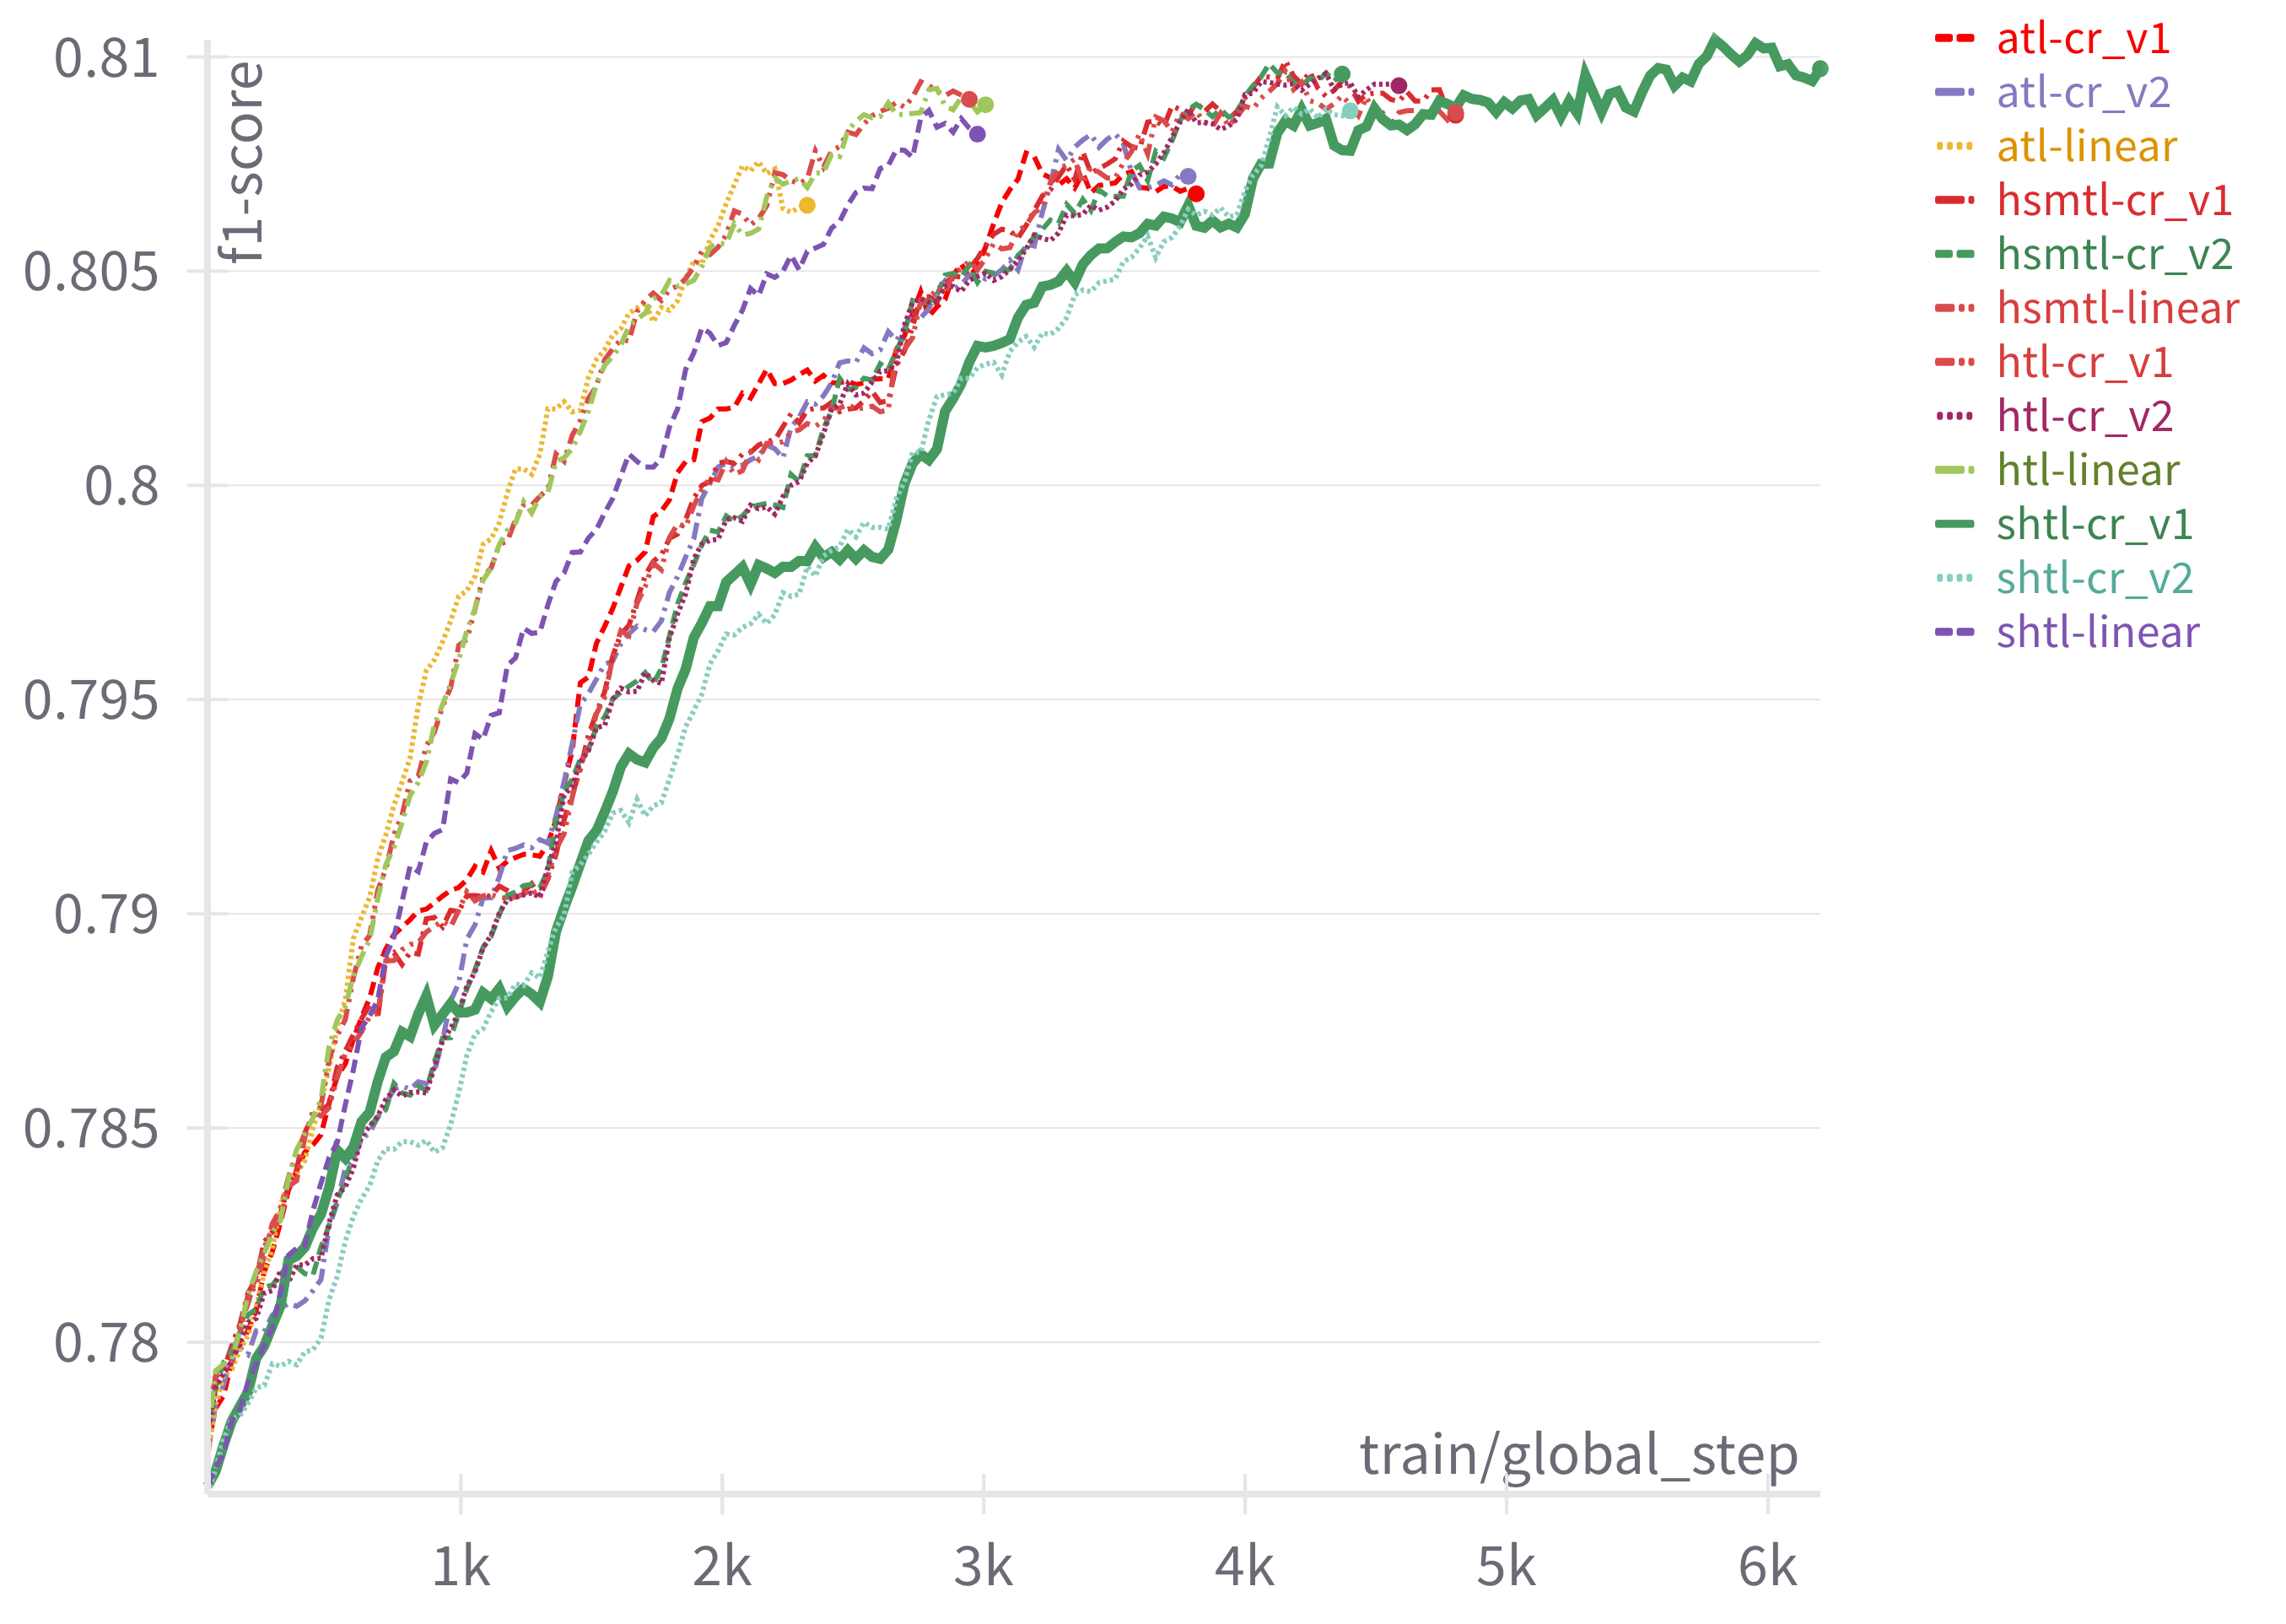
\includegraphics[scale=0.15,trim={0 0 0 0},clip]{Binary Classification Eval fine-tuning.png}
    \caption{Validation \(F_1\)-Score}
    % {\footnotesize Clockwise from bottom left: 4-class raw text, 3-class raw text, binary raw text, binary
    %     structured topics, 3-class structured topics, and 4-class structured topics.\\\footnotemark[1]ins: insufficient description}
    \label{fig:binaryf1}
\end{figure}

A visual inspection of the learning curves reveals several distinct patterns. The configurations utilizing \verb|BatchHardSoftMarginTripletLoss| seem to consistently demonstrate superior performance.  They exhibit some of the steepest learning curves, indicating faster convergence, and reach some of the highest peak \(F_1\)-scores, surpassing all loss function types.  The \verb|BatchHardTripletLoss| family of functions seem to perform similarly, albeit slightly worse. \verb|AllTripletLoss| configurations display the steepest learning curves, but show a performance collapse much earlier and at much lower \(F_1\)-score peaks than any of the other functions.  Finally, the \verb|BatchSemiHardTripletLoss| configurations exhibit the slowest learning curves, and do not seem to seem to reach the highest peak scores on average.  Nonetheless, it appears that its more erratic behavior near its plateau can produce results that surpass all other functions.  These visual trends strongly suggest that the choice of triplet mining strategy is a major factor in determining the training speed and final performance of the fine-tuned model for this task.

\subsubsection{Quantitative Performance Summary}
To provide a more precise and formal comparison, the exact peak validation \(F_1\)-scores achieved by each configuration are summarized in Table~\ref{tab:finetune_f1_scores}. This table distills the dynamic information from the learning curves into a single, quantitative metric for each experimental condition, enabling a direct and data-driven selection of the optimal configuration.
\begin{table}[tb]
    \captionsetup{skip=5pt}
    \centering
    \caption{Peak Validation F1-Score of Fine-Tuning Configurations on BGE Model}
    \label{tab:finetune_f1_scores}
    \resizebox{\columnwidth}{!}{
        \begin{tabular}{l c c c}
        \toprule
        \textbf{Loss Function} & \textbf{Linear Scheduler} & \textbf{Cosine Restarts v1} & \textbf{Cosine Restarts v2} \\
        \midrule
        \texttt{BatchAllTripletLoss} (atl) & 0.8076 & 0.8078 & 0.8082 \\
        \texttt{BatchHardSoftMarginTripletLoss} (hsmtl) & 0.8094 & 0.8099 & 0.8098 \\
        \texttt{BatchHardTripletLoss} (htl) & 0.8093 & 0.8097 & 0.8096 \\
        \texttt{BatchSemiHardTripletLoss} (shtl) & 0.8088 & \textbf{0.8104} & 0.8088 \\
        \bottomrule
        \end{tabular}
    }
\end{table}
The quantitative data presented in Table~\ref{tab:finetune_f1_scores} reveals a nuanced outcome that adds precision to the qualitative analysis of the learning curves. While the \verb|BatchHardTripletLoss| and \verb|BatchHardSoftMarginTripletLoss| configurations consistently achieved high scores across all schedulers, the single best-performing configuration was the combination of \verb|BatchSemiHardTripletLoss| and the \verb|cr_v1| learning rate schedule, which achieved the highest peak validation \(F_1\)-score of 0.8104. This result suggests that while aggressive hard-negative mining provides a strong and reliable performance floor, a more moderate semi-hard mining strategy, when paired with an appropriate cosine annealing schedule, can find a slightly better optimum for this specific task.

\section{Classifier Evaluation}

\section{Dimensionality Reduction}

\section{Comparative Analysis}

\section{Summary}

% shtl  cr2  0.808837656099904
% atl   cr1  0.8077551464982029
% atl   lin  0.8075537605064949
% shtl  cr1  0.8104033970276009
% hsmtl cr1  0.8099173553719007
% hsmtl cr2  0.8098371265235681
% shtl  lin  0.8087513340448239
% hsmtl lin  0.809419973833406
% atl   cr2  0.8082042330351299
% htl   cr1  0.8096584729171198
% htl   lin  0.8092648977816442
% htl   cr2  0.8096166341780376

